% Template CPE Lyon report
\documentclass[12pt, twosided]{cpe_report}

%%%%%%%%%%%%%%%%%%%%%%%%%%%%%%%%%%%%%%%%%%%%%%%%%
%%%%%%%%%%%%%%%% SETUP BEGINNING %%%%%%%%%%%%%%%%
%%%%%%%%%%%%%%%%%%%%%%%%%%%%%%%%%%%%%%%%%%%%%%%%%

% Do you want a bibliography? 
%(Comment on the next two lines if you don't want to)
\usepackage[style=ieee,backend=biber,hyperref=auto]{biblatex}
\addbibresource{references.bib}

% Color style of labels
\definecolor{MainColor}{RGB}{6,146,206} % CPE Blue Preset
%\definecolor{MainColor}{RGB}{0,62,116} % Imperial Blue Preset
%\definecolor{MainColor}{RGB}{6,206,86} % Green Preset
%\definecolor{MainColor}{RGB}{X,X,X} % Define your own color


% Language. Supported : fr, en 
\langage{en} % If you get an error when changing language, please clear the cache files.

% Main title
\maintitle{This is the main title}

% Subtitle
\subtitle{This is a subtitle}

% Author
\author{ % Will go under the section "Written by". Multiple authors allowed
    N.S. Surname \\[1mm]
    Mr. Surname2
}

% Supervisor
\supervisor{ % Will go under the section "Surpevised by". Multiple supervisor allowed
    Mr. Name \\[1mm]
    Prof. A. Another
}

% Current year of studies. Ex: 4ETI, 3CGP
\schoolyear{3ETI}

% [Optional] Duration of the work. 
\setboolean{set_duration}{true} %If you don't want to display it, set the bool set_duration to 'false'
\duration{01/01/2024}{31/12/2024}

% [Optional] Major. Ex: ESE
\setboolean{set_major}{true} %If you don't want to display it, set the bool set_major to 'false'
\major{ESE}

% [Optional] Address
\setboolean{set_address}{true} %If you don't want to display it, set the bool set_address to 'false'
\address{
City, \\
Address, \\
Postal Code, Country \\
}

% Do you want an abstract?
\setboolean{abstract}{true} % false or true - Default is true

% Do you want a list of figures?
\setboolean{list_of_figures}{true} % false or true - Default is true

% Do you want a list of tables?
\setboolean{list_of_tables}{true} % false or true - Default is true

% Do you want a mini list of tables for each chapter?
\setboolean{mini_list_of_tables}{true} % false or true - Default is true

% Do you want an acknowledgement page?
\setboolean{acknowledgement}{true} % false or true - Default is true

% Do you want a list of acronyms?
\setboolean{acronyms}{true} % false or true - Default is true

% Do you want a big chapter style ?
\setboolean{big_chapter_style}{false} % false or true - Default is false

% If you want to print your document, consider changing the command below to true. If true, the command adds labels at the edge of the pages which will make easy to identify a chapter running through the pages with the finger. It is just a visual setting.
\setboolean{edge_labels}{true} % false or true - Default is true

%%%%%%%%%%%%%%%%%%%%%%%%%%%%%%%%%%%%%%%%%%%%%%%%%
%%%%%%%%%%%%%%%% SETUP ENDING %%%%%%%%%%%%%%%%%%%
%%%%%%%%%%%%%%%%%%%%%%%%%%%%%%%%%%%%%%%%%%%%%%%%%

\begin{document}

\preamble

% ADD AS MANY CHAPTERS AS NEEDED
% BY CREATING .TEX FILES IN THE FOLDER chapters
% AND ADDING \input{namechapter.tex} BELOW
\chapter{Introduction}
\label{ch1}

%%%%%%%%%%%%%%%%%%%%%%%%%%%%%%%%%%%%%%%
% IMPORTANT
% THESE LINES MUST APPEAR IN EVERY CHAPTER
% COPY THEM IN ANY NEW CHAPTER
\begin{spacing}{1} 
\ifthenelse{\boolean{mini_list_of_tables}}{
    \minitoc 
}{}
\end{spacing}
\doublespacing 
%%%%%%%%%%%%%%%%%%%%%%%%%%%%%%%%%%%%%%%


\section{Title section}

Let's cite! The Einstein's journal paper \cite{einstein} and the Dirac's 
book \cite{dirac} are physics related items. 

And some acronyms: \ac{USA} and \ac{LTI} systems.

\begin{figure}
\centering
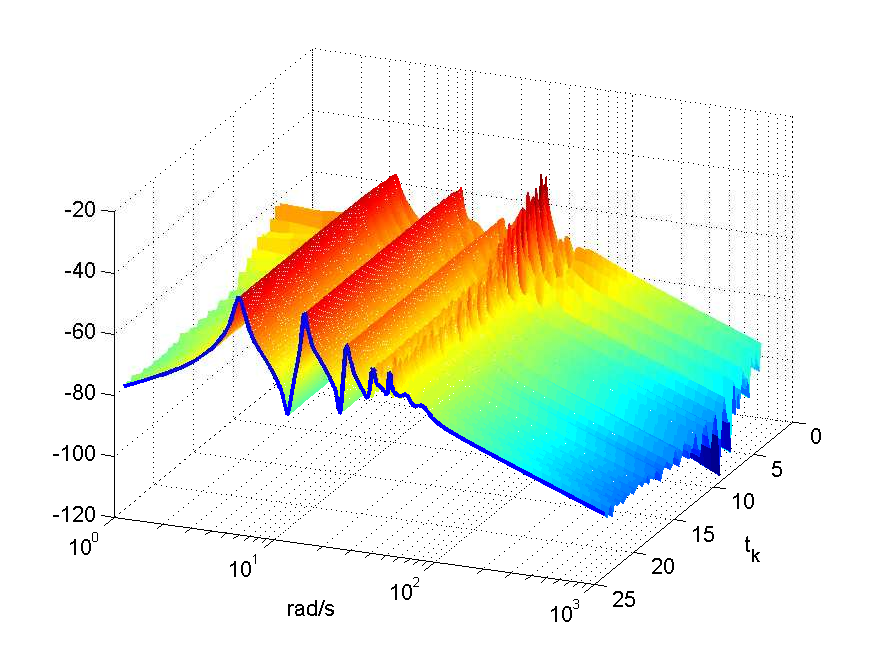
\includegraphics[width=0.8\columnwidth]{imgs/buildmagnitude.pdf}
\caption[Short description for list of figures]{This figure is taken from \cite{Sca:16}.}
\label{fig-magnitude}
\end{figure}%

\subsection{Title subsection}

\kant[1-6]

\chapter{Title chapter 2}
\label{ch2}

%%%%%%%%%%%%%%%%%%%%%%%%%%%%%%%%%%%%%%%
% IMPORTANT
% THESE LINES MUST APPEAR IN EVERY CHAPTER
% COPY THEM IN ANY NEW CHAPTER
\begin{spacing}{1} 
\ifthenelse{\boolean{mini_list_of_tables}}{
    \minitoc 
}{}
\end{spacing}
\doublespacing 
%%%%%%%%%%%%%%%%%%%%%%%%%%%%%%%%%%%%%%%

\kant[1]

\section{Title section 2.1}

\kant[1-3]

\conclusions
% EDIT THE CONTENT OF THE FILE
% Conclusions.tex
% You can find it under the folder 
% "chapters" on the left column


\RemoveLabels % Do not change - required
\printbibliography
%\printbibliography[title={Bibliographie}] % Use this line if you have choose 'fr' and comment previous one

\end{document}
